\documentclass{article}
%\usepackage[francais]{babel}
%\usepackage[utf8]{inputenc} % Required for including letters with accents
%\usepackage[T1]{fontenc} % Use 8-bit encoding that has 256 glyphs
\usepackage{pythontex}
\usepackage{amsthm}
\usepackage{amsmath}
\usepackage{amssymb}
\usepackage{mathrsfs}
\usepackage{graphicx}
\usepackage{geometry}
\usepackage{stmaryrd}
\usepackage{tikz}
\usetikzlibrary{patterns}
%\usetikzlibrary{intersections}
\usepackage[cache=false]{minted}
\usepackage{xcolor}

\usepackage{stmaryrd}
%\usetikzlibrary{tikzmark}
\usepackage{empheq}
\usepackage{longtable}
\usepackage{booktabs} 
\usepackage{array}
\usepackage{pstricks}
\usepackage{pst-3dplot}
\usepackage{pst-tree}
\usepackage{pstricks-add}
\usepackage{upgreek}
%\usepackage{epstopdf}
\usepackage{eolgrab}
\usepackage{chngpage}
 \usepackage{calrsfs}
 % Appel du package pythontex 
\usepackage{pythontex}

\usepackage{algorithm2e}
\RestyleAlgo{algoruled}
  \SetKw{KwFrom}{from} 
\newenvironment{algo}{
\begin{algorithm}[H]
\DontPrintSemicolon \SetAlgoVlined}
{\end{algorithm}}



\usetikzlibrary{decorations.pathmorphing}
\def \de {{\rm d}}
\usepackage{color}
\usepackage{xcolor}
\newcommand{\mybox}[1]{\fbox{$\displaystyle#1$}}
\newcommand{\myredbox}[1]{\fcolorbox{red}{white}{$\displaystyle#1$}}
\newcommand{\mydoublebox}[1]{\fbox{\fbox{$\displaystyle#1$}}}
\newcommand{\myreddoublebox}[1]{\fcolorbox{red}{white}{\fcolorbox{red}{white}{$\displaystyle#1$}}}

\usepackage{xcolor}
%\setbeamercolor{background canvas}{bg=lightgray}
\definecolor{LightGray}{gray}{0.9}
\definecolor{monOrange}{rgb}{0.97,0.35,0.04}
\usepackage{enumitem}
 \title{Les fonctionnalités avancées des composants}
\author{Ibrahim ALAME}
\date{14/02/2023}
\begin{document}
\maketitle

\section{Introduction au chapitre}
\subsection{Objectifs du chapitre}
Nous allons voir comment utiliser {\color{monOrange}v-model} sur les composants. Nous allons étudier les cascades d'attributs, les {\color{monOrange}slots}, l'injection avec {\color{monOrange}Provide} et {\color{monOrange}Inject}.

Nous verrons également des fonctions utilitaires permettant de transformer des objets réactifs en références. Enfin, nous verrons les composants asynchrones.

\subsection{Code de la vidéo}
Pour rappel, la directive {\color{monOrange}v-model} équivaut à l'utilisation de {\color{monOrange}v-bind} sur l'attribut value et de l'utilisation de {\color{monOrange}v-on} sur l'événement input. Voici l'équivalent de {\color{monOrange}v-model} :


%%%%%%%%%%%%%%%%%%%%%%%%%%%%%%%%%%%%%%%%%%%%%%%%%%%%%%%%%%%%%

\section{Utilisation de la directive v-model sur des composants}
\subsection{Fonctionnement de {\color{monOrange}v-model} avec un composant}
Lorsque vous utilisez {\color{monOrange}v-model} sur un composant enfant :
\begin{minted}[
mathescape,
framesep=2mm,
baselinestretch=1.2,
%fontsize=\footnotesize,
bgcolor=LightGray,
%linenos
]{html}
<Enfant v-model="uneProp" />
\end{minted}
Cela revient en fait exactement à :
\begin{minted}[
mathescape,
framesep=2mm,
baselinestretch=1.2,
%fontsize=\footnotesize,
bgcolor=LightGray,
%linenos
]{html}
<Enfant
  :modelValue="uneProp"
  @update:modelValue="val => uneProp = val"
/>
\end{minted}
Cela signifie que dans le composant enfant il faut émettre un événement {\color{monOrange}update:modelValue} et déclarer une {\color{monOrange}prop modelValue} :
\begin{minted}[
mathescape,
framesep=2mm,
baselinestretch=1.2,
%fontsize=\footnotesize,
bgcolor=LightGray,
%linenos
]{html}
<script setup>
defineProps<{
  modelValue: string;
}>();
defineEmits<{
  (e: 'update:modelValue', value: string);
}>();
</script>

<template>
  <input
    :value="modelValue"
    @input="$emit('update:modelValue', $event.target.value)"
  />
</template>
\end{minted}
\subsection{Changer le nom de la {\color{monOrange}prop} et de l'événement}
Comme nous venons de le voir, par défaut, la {\color{monOrange}prop} reçue par le composant enfant est {\color{monOrange}modelValue} et l'événement qu'il doit ressentir est {\color{monOrange}update:modelValue}. Il est possible de modifier le nom en passant un argument à {\color{monOrange}v-model} :
\begin{minted}[
mathescape,
framesep=2mm,
baselinestretch=1.2,
%fontsize=\footnotesize,
bgcolor=LightGray,
%linenos
]{html}
<Enfant v-model:unNom="uneProp" />
\end{minted}
Vous pouvez ensuite utiliser ce nom dans le composant enfant :
\begin{minted}[
mathescape,
framesep=2mm,
baselinestretch=1.2,
%fontsize=\footnotesize,
bgcolor=LightGray,
%linenos
]{html}
<script setup>
defineProps<{
  unNom: string;
}>();
defineEmits<{
  (e: 'update:unNom', value: string);
}>();
</script>

<template>
  <input
    type="text"
    :value="unNom"
    @input="$emit('update:unNom', $event.target.value)"
  />
</template>
\end{minted}
\subsection{Utiliser plusieurs directives {\color{monOrange}v-model}}
Vous pouvez sans problème utiliser plusieurs directives v-model sur un composant :
\begin{minted}[
mathescape,
framesep=2mm,
baselinestretch=1.2,
%fontsize=\footnotesize,
bgcolor=LightGray,
%linenos
]{html}
<Enfant v-model:une-prop="uneProp" v-model:une-autre-prop="uneAUtreProp" />
\end{minted}
Par exemple :
\begin{minted}[
mathescape,
framesep=2mm,
baselinestretch=1.2,
%fontsize=\footnotesize,
bgcolor=LightGray,
%linenos
]{html}
<Modal v-model:prenom="prenom" v-model:nom="nom" />
\end{minted}
Et nous aurions dans le composant enfant :
\begin{minted}[
mathescape,
framesep=2mm,
baselinestretch=1.2,
%fontsize=\footnotesize,
bgcolor=LightGray,
%linenos
]{html}
<template>
  <input
    type="text"
    :value="prenom"
    @input="$emit('update:prenom', $event.target.value)"
  />
  <input
    type="text"
    :value="nom"
    @input="$emit('update:nom', $event.target.value)"
  />
</template>

<script setup lang="ts">
defineProps<{
  prenom: string;
  nom: string;
}>();

defineEmits<{
  (e: 'update:prenom', value: string);
  (e: 'update:nom', value: string);
}>();
</script>

<style scoped lang="scss"></style>
\end{minted}
Voici l'exemple exécutable :


\subsection{Utiliser des modificateurs}
Vous pouvez utiliser des modificateurs personnalisés ou définis par {\color{monOrange}Vue.js}, comme par exemple {\color{monOrange}trim, number} etc. Par exemple, pour supprimer les espaces possibles avant ou après :
\begin{minted}[
mathescape,
framesep=2mm,
baselinestretch=1.2,
%fontsize=\footnotesize,
bgcolor=LightGray,
%linenos
]{html}
<Modal v-model:prenom.trim="prenom" v-model:nom.trim="nom" />
\end{minted}
Pour utiliser un modificateur personnalisé, il faut utiliser côté parent :
\begin{minted}[
mathescape,
framesep=2mm,
baselinestretch=1.2,
%fontsize=\footnotesize,
bgcolor=LightGray,
%linenos
]{html}
<Modal v-model:prenom="prenom" v-model:nom.exemple="nom" />
\end{minted}
Et côté enfant :
\begin{minted}[
mathescape,
framesep=2mm,
baselinestretch=1.2,
%fontsize=\footnotesize,
bgcolor=LightGray,
%linenos
]{html}
<template>
  <input
    type="text"
    :value="prenom"
    @input="$emit('update:prenom', $event.target.value)"
  />
  <input
    type="text"
    :value="nom"
    @input="emitName"
  />
</template>

<script setup lang="ts">
defineProps<{
  prenom: string;
  nom: string;
  nameModifiers?: { [s: string]: boolean };
}>();

defineEmits<{
  (e: 'update:prenom', value: string);
  (e: 'update:nom', value: string);
}>();

function emitName(event) {
  let value = (event.target as HTMLInputElement).value;
  if (props.modelModifiers.exemple) {
    // Modifier la valeur comme on souhaite si le modificateur est présent :
    value = value.toUpperCase();
  }
  emit('update:modelValue', value);
}
</script>

<style scoped lang="scss"></style>
\end{minted}
\subsection{Code de la vidéo}
Pour rappel, la directive {\color{monOrange}v-model} équivaut à l'utilisation de {\color{monOrange}v-bind} sur l'attribut value et de l'utilisation de {\color{monOrange}v-on} sur l'événement {\color{monOrange}input}. Voici l'équivalent de {\color{monOrange}v-model} :

%%%%%%%%%%%%%%%%%%%%%%%%%%%%%%%%%%%%%%%%%%%%%%%%%%%%%%%%%%%%%%%


\section{Cascade d'attributs}
\subsection{Les attributs en cascade}
{\em Les attributs en cascade sont rarement utilisés, vous pouvez passer rapidement pour une première approche de {\color{monOrange}Vue.js} et y revenir plus tard.}

Un attribut en cascade est un attribut ou un écouteur d'événement déclaré avec {\color{monOrange}v-on} qui est passé à un composant sans être déclaré précisé, c'est-à- dire sans utiliser de {\color{monOrange}props}. Par exemple, si nous avons le composant enfant :
\begin{minted}[
mathescape,
framesep=2mm,
baselinestretch=1.2,
fontsize=\footnotesize,
bgcolor=LightGray,
%linenos
]{html}
<template>
  <h1>Hello</h1>
</template>
\end{minted}
Et que nous déclarons un attribut sur celui-ci dans le composant parent :
\begin{minted}[
mathescape,
framesep=2mm,
baselinestretch=1.2,
fontsize=\footnotesize,
bgcolor=LightGray,
%linenos
]{html}
<template>
  <Enfant class="large" />
</template>
\end{minted}
Le composant enfant rendu sur le DOM sera :
\begin{minted}[
mathescape,
framesep=2mm,
baselinestretch=1.2,
fontsize=\footnotesize,
bgcolor=LightGray,
%linenos
]{html}
<h1 class="large">Hello</h1>
\end{minted}
\subsection{Fusionnement d'attributs}
Comme vu précédemment, si le composant enfant a déjà un attribut déclaré, les valeurs seront fusionnées. En reprenant l'exemple avec l'attribut {\color{monOrange}class} :
\begin{minted}[
mathescape,
framesep=2mm,
baselinestretch=1.2,
fontsize=\footnotesize,
bgcolor=LightGray,
%linenos
]{html}
<template>
  <h1 class="titre">Hello</h1>
</template>
\end{minted}
Et dans le composant parent :
\begin{minted}[
mathescape,
framesep=2mm,
baselinestretch=1.2,
fontsize=\footnotesize,
bgcolor=LightGray,
%linenos
]{html}
<template>
  <Enfant class="large" />
</template>
\end{minted}
Nous aurons :
\begin{minted}[
mathescape,
framesep=2mm,
baselinestretch=1.2,
fontsize=\footnotesize,
bgcolor=LightGray,
%linenos
]{html}
<h1 class="titre large">Hello</h1>
\end{minted}
\subsection{Ecouteurs déclarés avec {\color{monOrange}v-on}}
C'est exactement le même principe avec les écouteurs d'événements déclarés en utilisant {\color{monOrange}v-on}. Si le {\color{monOrange}template} du composant parent est :
\begin{minted}[
mathescape,
framesep=2mm,
baselinestretch=1.2,
fontsize=\footnotesize,
bgcolor=LightGray,
%linenos
]{html}
<template>
  <Enfant @click="onClick" />
</template>
<script>
function onClick() {
  console.log("clic");
}
</script>
\end{minted}
L'écouteur sera placé automatiquement sur l'élément racine du composant enfant. Un clic sur le composant enfant déclenchera donc le gestionnaire déclaré dans le composant parent. A noter que si l'élément racine du composant enfant a déjà un ou plusieurs gestionnaires d'événements déclarés, ils seront également exécutés. Cela ne les remplacera pas.

\subsection{Utilisation de {\color{monOrange}\$attrs} côté {\color{monOrange}template}}
{\color{monOrange}Vue} met à disposition automatiquement une propriété {\color{monOrange}\$attrs} que vous pouvez utiliser dans le {\color{monOrange}template} du composant enfant. Elle contient tous les attributs et les écouteurs d'événements passés en cascade. C'est par exemple utile si le composant enfant n'a pas d'élément racine, pour décider de placer les attributs reçus sur un élément particulier :
\begin{minted}[
mathescape,
framesep=2mm,
baselinestretch=1.2,
fontsize=\footnotesize,
bgcolor=LightGray,
%linenos
]{html}
<template>
  <h1>Hello</h1>
  <h2 v-bind="$attrs">Hello 2</h2>
</template>
\end{minted}
\subsection{Utilisation de {\color{monOrange}useAttrs()} côté {\color{monOrange}script}}
Il est également possible d'accéder aux attributs en utilisant {\color{monOrange}useAttrs()} cîoté {\color{monOrange}script} :
\begin{minted}[
mathescape,
framesep=2mm,
baselinestretch=1.2,
fontsize=\footnotesize,
bgcolor=LightGray,
%linenos
]{html}
<script setup>
  
import { useAttrs } from 'vue';

const attrs = useAttrs();
</script>
\end{minted}
\subsection{Désactivation du passage automatique des attributs}
Il est possible de désactiver le passage automatique des attributs dans le cas où par exemple, vous avez bien un élément racine sur le composant enfant mais que vous souhaitez appliquer les attributs sur d'autres éléments :
\begin{minted}[
mathescape,
framesep=2mm,
baselinestretch=1.2,
fontsize=\footnotesize,
bgcolor=LightGray,
%linenos
]{html}
<template>
  <div class="uneClasse">
    <h1>Hello</h1>
    <h2 v-bind="$attrs">Hello 2</h2>
  </div>
</template>

<script lang="ts">
export default {
  inheritAttrs: false,
};
</script>

<script setup lang="ts"></script>
\end{minted}
Notez bien l'utilisation de deux balises {\color{monOrange}scripts} ! Elles seront fusionnées automatiquement avec la configuration par {\color{monOrange}Vite}.

\subsection{Code de la vidéo}
Voici le code de la vidéo :

%%%%%%%%%%%%%%%%%%%%%%%%%%%%%%%%%%%%%%%%%%%%%%%%%%%%%%%%%%%%%

\section{Présentation des slots}
\subsection{Les {\color{monOrange}slots}}
Les {\color{monOrange}slots} permettent de passer des parties de {\color{monOrange}template} d'un composant parent à un composant enfant. Nous avions vu les {\color{monOrange}props} qui permettent de passer des valeurs JavaScript d'un composant parent à un composant enfant.

Les {\color{monOrange}slots} permettent de passer du HTML. Pour utiliser les {\color{monOrange}slots}, il faut utiliser le composant enfant avec deux balises et mettre le fragment HTML à passer, c'est-à -dire le {\color{monOrange}slot}, entre ces deux balises :
\begin{minted}[
mathescape,
framesep=2mm,
baselinestretch=1.2,
fontsize=\footnotesize,
bgcolor=LightGray,
%linenos
]{html}
<Enfant>
  J’insère du contenu ici pour le passer au composant enfant.
</Enfant>
\end{minted}
Dans le composant enfant, il faut utiliser une balise {\color{monOrange}<slot>} pour indiquer où afficher le contenu passé :
\begin{minted}[
mathescape,
framesep=2mm,
baselinestretch=1.2,
fontsize=\footnotesize,
bgcolor=LightGray,
%linenos
]{html}
<template>
  // Le contenu sera projeté à la place de slot :
  <slot></slot>
</template>
\end{minted}
Voici le schéma officiel pour les {\color{monOrange}slots} avec un autre exemple simple :
\begin{center}
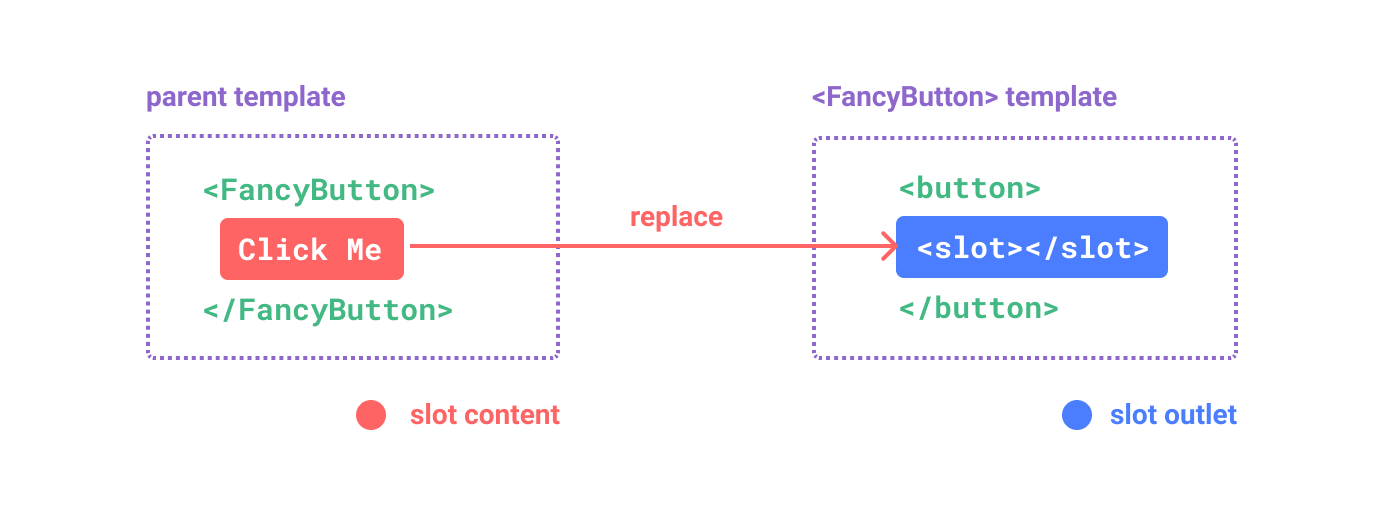
\includegraphics[width=10cm]{images/image10.png}
\end{center}

Dans le {\color{monOrange}template} du parent nous déclarons le fragment HTML à passer : en l'occurrence simplement le texte {\color{monOrange}Click Me}. Nous déclarons le contenu entre les balises du composant enfant {\color{monOrange}FancyButton}.

Dans le composant enfant, nous utilisons les balises {\tt <slot>} pour indiquer où insérer le contenu passé, dans l'occurrence le texte {\color{monOrange}Click Me}. Le rendu final sur le DOM sera donc :
\begin{minted}[
mathescape,
framesep=2mm,
baselinestretch=1.2,
fontsize=\footnotesize,
bgcolor=LightGray,
%linenos
]{html}
<button>
  Click Me
</button>
\end{minted}
Il est possible de passer n'importe quel contenu HTML comme par exemple une {\color{monOrange}div} :
\begin{minted}[
mathescape,
framesep=2mm,
baselinestretch=1.2,
fontsize=\footnotesize,
bgcolor=LightGray,
%linenos
]{html}
<template>
  <Enfant>
    <div>
      J’insère du contenu ici pour le passer au composant enfant.
    </div>
  </Enfant>
</template>
\end{minted}
Il est même possible de passer un autre composant :
\begin{minted}[
mathescape,
framesep=2mm,
baselinestretch=1.2,
fontsize=\footnotesize,
bgcolor=LightGray,
%linenos
]{html}
<template>
  <Enfant>
    <AutreComposant></AutreComposant>
  </Enfant>
</template>
\end{minted}
Le composant sera également remplacé à l'endroit de {\color{monOrange}slot}.

\subsection{Portée des variables}
Le contenu déclaré dans le composant parent a accès aux propriétés du composant parent :
\begin{minted}[
mathescape,
framesep=2mm,
baselinestretch=1.2,
fontsize=\footnotesize,
bgcolor=LightGray,
%linenos
]{html}
<template>
  <span>{{ message }}</span>
  <Enfant>{{ message }}</Enfant>
</template>
\end{minted}
Ici si le composant parent a une propriété {\color{monOrange}message} côté {\color{monOrange}script}, aucun problème pour l'utiliser dans le contenu à passer en {\color{monOrange}slot} au composant enfant.

En revanche, le contenu n'a pas accès par défaut aux propriétés du composant enfant. Donc dans notre exemple, si la propriété {\color{monOrange}message} était déclarée dans le composant enfant, nous aurions une erreur.

\subsection{Les {\color{monOrange}slots} nommés}
Il est parfois nécessaire de projeter plusieurs contenus à des endroits précis. Dans ce cas, il faut utiliser plusieurs éléments {\color{monOrange}slot} et les identifiants de manière unique. Pour nommer un {\color{monOrange}slot} côté composant parent, il suffit d'utiliser la directive {\color{monOrange}v-slot} sur l'élément projeté et de lui passer l'identifiant :
\begin{minted}[
mathescape,
framesep=2mm,
baselinestretch=1.2,
fontsize=\footnotesize,
bgcolor=LightGray,
%linenos
]{html}
<template>
  <Enfant>
    <h1 v-slot:header>Titre de mon site</h1>
    <p v-slot:footer>Qui sommes-nous ?</p>
  </Enfant>
</template>
\end{minted}
La notation raccourcie de la directive {\color{monOrange}v-slot} est {\color{monOrange}\#}, nous pouvons donc faire :
\begin{minted}[
mathescape,
framesep=2mm,
baselinestretch=1.2,
fontsize=\footnotesize,
bgcolor=LightGray,
%linenos
]{html}
<template>
  <Enfant>
    <h1 #header>Titre de mon site</h1>
    <p v-#footer>Qui sommes-nous ?</p>
  </Enfant>
</template>
\end{minted}
Dans notre exemple nous avons défini deux {\color{monOrange}slot header} et {\color{monOrange}footer} qui nous permettent de référencer les contenus à projeter. Dans le composant enfant, il suffit d'utiliser l'attribut {\color{monOrange}name} sur un {\color{monOrange}slot} pour indiquer que le contenu référencé doit être projeté à cet endroit :
\begin{minted}[
mathescape,
framesep=2mm,
baselinestretch=1.2,
fontsize=\footnotesize,
bgcolor=LightGray,
%linenos
]{html}
<template>
  <header>
    <slot name="header"></slot>
  </header>
  <footer>
    <slot name="footer"></slot>
  </footer>
<template>
\end{minted}
Il est également possible de créer des identifiants dynamiques pour les {\color{monOrange}slots} dans les composants parents :
\begin{minted}[
mathescape,
framesep=2mm,
baselinestretch=1.2,
fontsize=\footnotesize,
bgcolor=LightGray,
%linenos
]{html}
<template v-slot:[nomDynamique]>
    Du contenu HTML
</template>
\end{minted}
Vous pouvez également utiliser la notation raccourcie :
\begin{minted}[
mathescape,
framesep=2mm,
baselinestretch=1.2,
fontsize=\footnotesize,
bgcolor=LightGray,
%linenos
]{html}
<template #[nomDynamique]>
  Du contenu HTML
</template>
\end{minted}
\subsection{Contenu par défaut}
Il est également possible de définir un contenu par défaut si aucun contenu n'est passé.

Il suffit de mettre du contenu par défaut entre les balises {\tt <slot>} dans le composant enfant pour que celui-ci soit considéré comme contenu par défaut :
\begin{minted}[
mathescape,
framesep=2mm,
baselinestretch=1.2,
fontsize=\footnotesize,
bgcolor=LightGray,
%linenos
]{html}
<template>
  <slot name="header">Mon titre par défaut si aucun contenu n’est passé</slot>
<template>
\end{minted}
\subsection{Code de la vidéo}
Voici le code de la vidéo :

%%%%%%%%%%%%%%%%%%%%%%%%%%%%%%%%%%%%%%%%%%%%%%%%%%%%%%%%%%%%%%

\section{Portes des machines à sous}
\subsection{Passer des données aux slots}
Nous avons vu que par défaut, le contenu des {\color{monOrange}slots} ne peut accéder aux propriétés déclarées dans le composant enfant.

Il est cependant possible de passer des valeurs aux contenus des {\color{monOrange}slots} depuis le composant enfant. Pour ce faire, il faut passer des attributs aux {\color{monOrange}slots}, exactement de la même manière que pour les {\color{monOrange}props} aux composants. Bien sûr, cette fois-ci nous sommes dans le composant enfant :
\begin{minted}[
mathescape,
framesep=2mm,
baselinestretch=1.2,
fontsize=\footnotesize,
bgcolor=LightGray,
%linenos
]{html}
<div>
  <slot :prop="uneValeur" :autreProp="42"></slot>
</div>
\end{minted}
Dans le composant parent, nous pouvons utiliser ces propriétés passées depuis le composant enfant dans les contenus :
\begin{minted}[
mathescape,
framesep=2mm,
baselinestretch=1.2,
fontsize=\footnotesize,
bgcolor=LightGray,
%linenos
]{html}
<Enfant v-slot="slotProps">
  {{ slotProps.prop }} {{ slotProps.autreProp }}
</Enfant>
\end{minted}
Cela fonctionne également avec les {\color{monOrange}slots} nommés :
\begin{minted}[
mathescape,
framesep=2mm,
baselinestretch=1.2,
fontsize=\footnotesize,
bgcolor=LightGray,
%linenos
]{html}
<Enfant>
  <template #header="headerProps">
    {{ headerProps }}
  </template>

  <template #default="defaultProps">
    {{ defaultProps }}
  </template>

  <template #footer="footerProps">
    {{ footerProps }}
  </template>
</Enfant>
\end{minted}
Dans le composant enfant :
\begin{minted}[
mathescape,
framesep=2mm,
baselinestretch=1.2,
fontsize=\footnotesize,
bgcolor=LightGray,
%linenos
]{html}
<slot name="header" :uneProp="uneValeur"></slot>

<slot name="footer" :uneProp2="autreVal"></slot>
\end{minted}
\subsection{Code de la vidéo}
Voici le code de la vidéo :

%%%%%%%%%%%%%%%%%%%%%%%%%%%%%%%%%%%%%%%%%%%%%%%%%%%%%%%%%%%%%%

\section{Provide et Inject}
\subsection{Passer des données à travers plusieurs composants}
Supposons que vous vouliez passer des données à des composants enfants éloignés dans l'arbre. Vous pouvez utiliser des {\color{monOrange}props} sur plusieurs niveaux :
\begin{center}
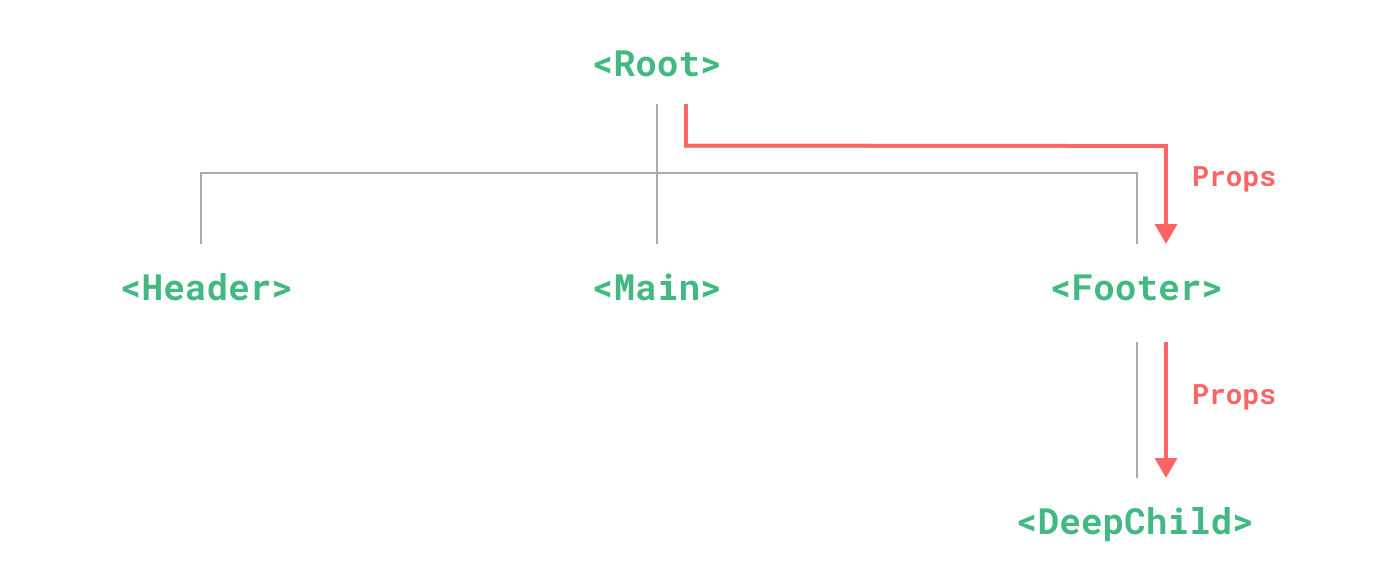
\includegraphics[width=10cm]{images/image11.png}
\end{center}

C'est d'ailleurs ce que nous avons fait dans le projet. Mais supposons que les composants ciblés soient à 3 ou 4 voir plus niveaux du composant contenant les données et que les composants intermédiaires n'étaient pas besoin de ces données. Comment faire pour passer des données sans devoir déclarer les mêmes {\color{monOrange}props} dans tous les composants ancêtres des composants cibles ? C'est là qu'interviennent {\color{monOrange}provide} et {\color{monOrange}inject} :
\begin{center}
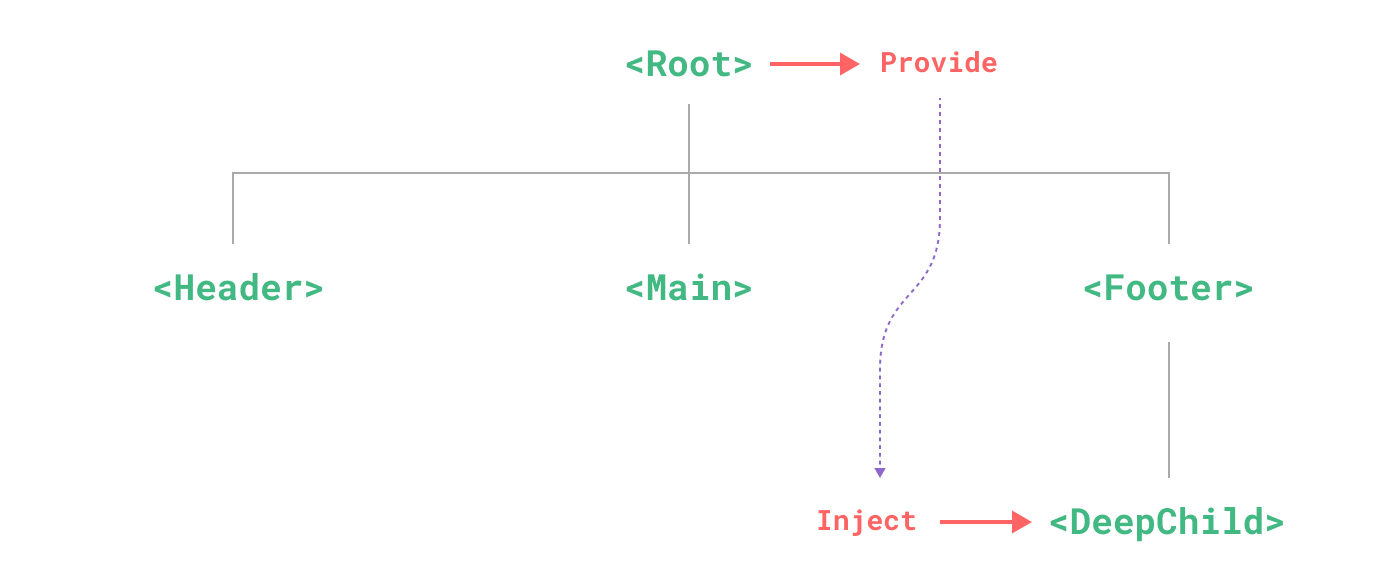
\includegraphics[width=10cm]{images/image12.png}
\end{center}

\subsection{La fonction {\color{monOrange}provide()}}
La fonction {\color{monOrange}provide()} permet de mettre à disposition des données réactives ou non à tous les composants descendants du composant l'utilisant. La syntaxe est :
\begin{minted}[
mathescape,
framesep=2mm,
baselinestretch=1.2,
fontsize=\footnotesize,
bgcolor=LightGray,
%linenos
]{html}
<script setup>
import { provide } from 'vue';

provide('clé', valeur);
</script>
\end{minted}
La clé d'injection doit être une chaîne de caractères mais la valeur peut être une valeur en dur ou une propriété réactive :
\begin{minted}[
mathescape,
framesep=2mm,
baselinestretch=1.2,
fontsize=\footnotesize,
bgcolor=LightGray,
%linenos
]{javascript}
import { ref, provide } from 'vue';

const compteur = ref(0);
provide('compteur', compteur);
\end{minted}
\subsection{Fournir des valeurs globalement}
Pour fournir des données à toute l'application et non seulement aux composants descendants d'un composant, vous pouvez utiliser la méthode provide() sur app dans main.ts :
\begin{minted}[
mathescape,
framesep=2mm,
baselinestretch=1.2,
fontsize=\footnotesize,
bgcolor=LightGray,
%linenos
]{html}
import { createApp } from 'vue';
import App from './App.vue';

const app = createApp(App);

app.provide('API_URL', 'https://restapi.fr/api');

app.mount('#app');
\end{minted}
\subsection{Injecter les données avec la fonction {\color{monOrange}inject()}}
La fonction {\color{monOrange}inject()} permet de récupérer les données fournies par {\color{monOrange}provide} dans un composant descendant :
\begin{minted}[
mathescape,
framesep=2mm,
baselinestretch=1.2,
fontsize=\footnotesize,
bgcolor=LightGray,
%linenos
]{html}
<script setup>
import { inject } from 'vue';

const compteur = inject('compteur');
</script>
\end{minted}
Comme nous utilisons {\color{monOrange}TypeScript}, il faut taper la valeur reçue en utilisant un type générique :
\begin{minted}[
mathescape,
framesep=2mm,
baselinestretch=1.2,
fontsize=\footnotesize,
bgcolor=LightGray,
%linenos
]{html}
const compteur = inject<number>('compteur');
\end{minted}
En effet, sans ça {\color{monOrange}TypeScript} n'a aucun moyen de savoir le type de la valeur retournée par la fonction {\color{monOrange}inject()}.

Lorsque vous êtes certain que la valeur fournie par {\color{monOrange}provide()} sera présente, et qu'elle ne peut donc pas être undefined, vous pouvez l'indiquer à {\color{monOrange}TypeScript} en utilisant ! :
\begin{minted}[
mathescape,
framesep=2mm,
baselinestretch=1.2,
fontsize=\footnotesize,
bgcolor=LightGray,
%linenos
]{html}
const compteur = inject<number>('compteur')!;
\end{minted}
\subsection{Modification des propriétés réactives}
Lorsque vous utilisez {\color{monOrange}provide/inject}, il est recommandé de laisser toutes les modifications des propriétés réactives dans le composant qui utilise {\color{monOrange}provide()}. Autrement dit, retenez la règle qu'il est interdit de modifier une propriété réactive fournie par {\color{monOrange}provide()} dans un composant descendant et qu'il faut le faire dans le composant parent.

{\color{monOrange}Vue.js} met à disposition la fonction {\color{monOrange}readonly()} pour ne pas oublier de respecter cette règle. Si vous voulez modifier des propriétés réactives depuis un composant enfant il faut passer une fonction avec {\color{monOrange}provide} qui sera appelée par le composant enfant :
\begin{minted}[
mathescape,
framesep=2mm,
baselinestretch=1.2,
fontsize=\footnotesize,
bgcolor=LightGray,
%linenos
]{html}
<script setup>
import { provide, ref, readonly } from 'vue';

const ville = ref('Paris');

function majVille() {
  ville.value = 'Nice';
}

provide('ville', readonly({
  ville,
  majVille
}));
</script>
\end{minted}
Et dans le composant descendant :
\begin{minted}[
mathescape,
framesep=2mm,
baselinestretch=1.2,
fontsize=\footnotesize,
bgcolor=LightGray,
%linenos
]{html}
<script setup>
import { inject } from 'vue';

const { ville, majVille } = inject<{ ville: string; majVille: () => void }>('ville');
</script>

<template>
  <button @click="majVille">{{ ville }}</button>
</template>
\end{minted}
\subsection{Code de la vidéo}
Voici le code de la vidéo :




\end{document}


\begin{minted}[
mathescape,
framesep=2mm,
baselinestretch=1.2,
fontsize=\footnotesize,
bgcolor=LightGray,
%linenos
]{html}

\end{minted}